\begin{tikzpicture}[scale=.5]
	\node[anchor=south west, inner sep=0] (image) at (0,0) {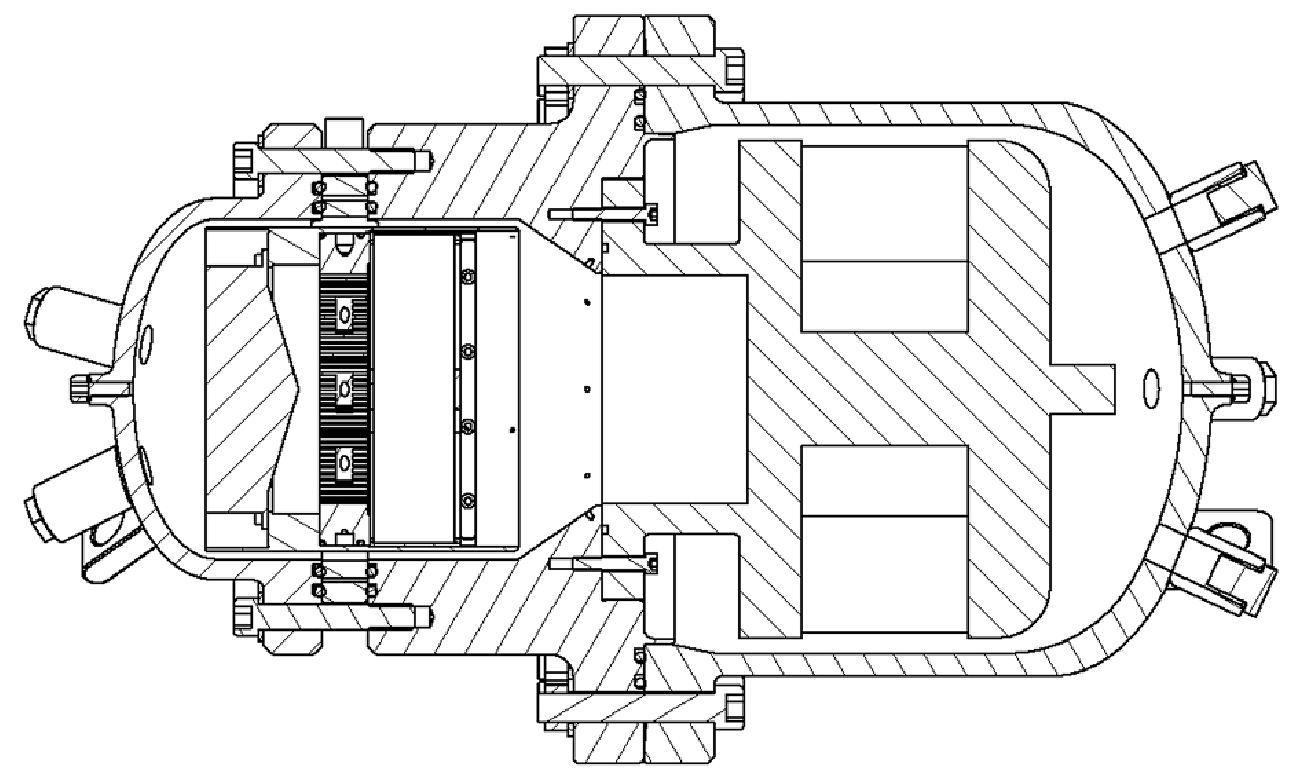
\includegraphics[angle=0,origin=c,width=.6\textwidth]{../fig/fig_TACOTSchematics/TACOT.png}};
	
	\node[anchor=east, inner sep=0] (imagecropped) at (image.west) {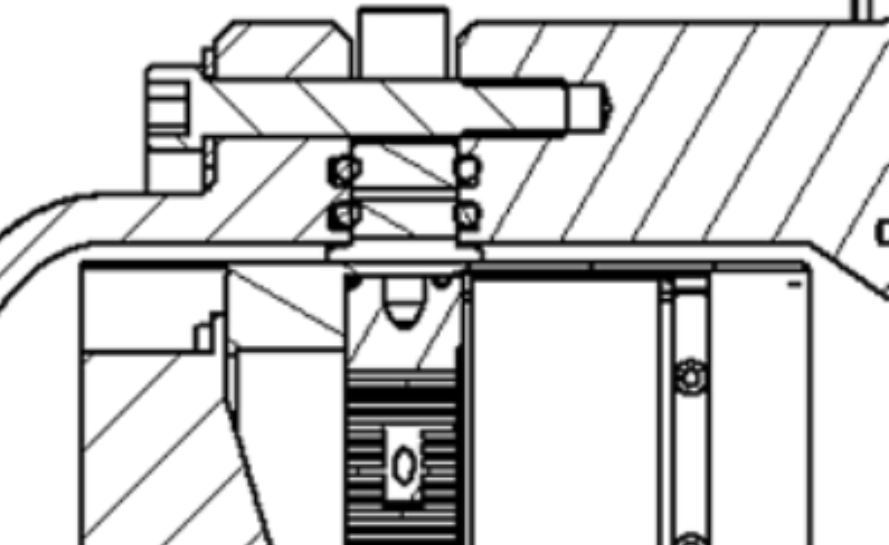
\includegraphics[angle=0,origin=c,width=.35\textwidth]{../fig/fig_TACOTSchematics/TACOT_Cropped.png}};

\draw[black, very thick, dashed, rounded corners] (imagecropped.north west) rectangle (imagecropped.south east);
%\draw[black, very thick, dashed, rounded corners] ($(AHX)+(-1.5cm,3cm)$) rectangle ($(CHX)+(.75cm,-.5cm)$);
	
	\begin{scope}[x={(image.south east)},y={(image.north west)}]
	
%		\filldraw (0,0) circle (2pt); 
%		\filldraw[green] (1,0) circle (1pt);
%		\filldraw[red] (1,1) circle (1pt);		
%		\filldraw[blue] (0,1) circle (1pt);
%		\draw[help lines,xstep=.1,ystep=.1] (0,0) grid (1,1);
%		\fill[orange, rounded corners, opacity=1,draw=orange] (.46,.65) -- ++(132:.09) -- ++(0,-.44) -- ++(48:.09) -- cycle;
		\draw[MatlabYellow,rounded corners,very thick,preaction={fill=MatlabYellow!20,opacity=.5}] (.46,.65) -- ++(132:.09) -- ++(-.03,0) -- ++(0,-.44) --++(.03,0) -- ++(48:.09) -- cycle; %node[left,pos=.5,label={[rotate=90]center:Cavité}]{};
		\draw[MatlabYellow] (.415,0.5) node [label={[rotate=90]center:\textbf{Cône}}]{};
		
%		\draw[blue] (.5,.5) node [anchor=center, preaction={fill=black!20,opacity=.7}] {RIX};
%		\draw[red] (.33,.5) node [anchor=center, preaction={fill=black!20,opacity=.7}] {TA core};	
	
		\draw[MatlabPurple,rounded corners,very thick,preaction={fill=MatlabPurple!20,opacity=.5}] (.365,.7) rectangle (.245,.3) node[pos=.5,label={[rotate=90]center:\textbf{Noyau}}]{};
		
		\node (AHX) at (.27,.65) {};
		\node (Reg) at (.32,.65) {};
		\node (CHX) at (.36,.65) {};
		\node (RIX) at (.77,.4) {};

		\node (HP) at (.19,.4) {};
		
		\draw[<-,very thick,MatlabOrange] (AHX.center) to[out=90,in=0] ($(AHX)+(-.2,.41)$) node[left]{\begin{tabular}{r} Echangeur de chaleur ambiant \\ (HXA) \end{tabular}};		
		\draw[<-,very thick] (Reg.center) to ($(Reg)+(0,.4)$) node[above]{Régénérateur};
		\draw[<-,very thick,MatlabBlue] (CHX.center) to[out=90,in=180] ($(CHX)+(.2,.41)$) node[right]{\begin{tabular}{l} Echangeur de chaleur froid \\ (HXF) \end{tabular}};
		
		\draw[->,very thick,green!50!black] ($(RIX)+(0,-.4)$) -- (RIX.center) node[pos=0,anchor=north]{\begin{tabular}{c}Source acoustique principale \\ (SA1) \end{tabular}};
		\draw[->,very thick,green!50!black] ($(HP)+(0,-.4)$) -- (HP.center) node (SA2) [pos=0,anchor=north]{\begin{tabular}{c}Source acoustique secondaire \\ (SA2) \end{tabular}};
		
%		\draw [white] (.455,.5) node{+};
%		\draw [white] (.41,.65) node{+};
%		\draw [white] (.41,.5) node{+};
%		\draw [white] (.41,.35) node{+};

		\draw[black, very thick, dashed, rounded corners] ($(AHX)+(-.14,.2)$) node(a){} rectangle ($(CHX)+(.07,-.1)$);
		
		\draw[black, very thick, dashed] (a) -- (imagecropped.north east);
		\draw[black, very thick, dashed] ($(a)+(0,-.3)$) -- (imagecropped.south east);
		

	\end{scope}
	
	\draw(imagecropped.south) node[below]{\small \textbf{(a)}};		
	\draw(SA2.south -| image.south) node{\small \textbf{(b)}};
	
\end{tikzpicture}